\documentclass[11pt]{article}

% Packages
\usepackage{amsmath, amsthm, amssymb}
\usepackage{hyperref}
\usepackage{graphicx}
\usepackage[utf8]{inputenc}
\usepackage{geometry}
\geometry{a4paper, margin=1in}

% Theorem Environments
\newtheorem{theorem}{Theorem}
\newtheorem{remark}{Remark}
\newtheorem{lemma}[theorem]{Lemma}
\newtheorem{corollary}[theorem]{Corollary}
\newtheorem{definition}[theorem]{Definition}
\newtheorem{proposition}[theorem]{Proposition}

% Document Information
\title{{\Large Cryptography meets algorithms (15893) Lecture Notes}\\[5pt]
{\bf Lecture 12: Oblivious Data Structures}}
\author{Scribe: Tanisha Saxena}
\date{\today}

\usepackage{caption}
\usepackage{subcaption}

\begin{document}

\maketitle

\section{Motivation}
In previous lectures, we learned how ORAM allows up to compile any program into an oblivious counterpart by simply using ORAM instead of RAM. However, this sort of generic application can cause unnecessarily high overhead. For example, in previous lectures we saw how ORAM could be used on sorting which caused $O(\log n)$ overhead. Instead, we can actually use the non-recursive tree idea from Path ORAM  to create oblivious data structures that allow us to more easily create oblivious protocols with lower overhead \cite{stefanov2018path}.

\section{Background}
Recall the recursive tree data structure used in Path ORAM \cite{stefanov2018path}. In this protocol, the client stores a small local stash. The server-side storage is treated as a tree of buckets where each block is stored in a random leaf and the unique path from the root to said leaf contains all the blocks not in the client stash. An access to Path ORAM can be described by the simple pseudocode shown in Figure \ref{fig:pathORAMpseudo}.

\begin{figure}
    \centering
    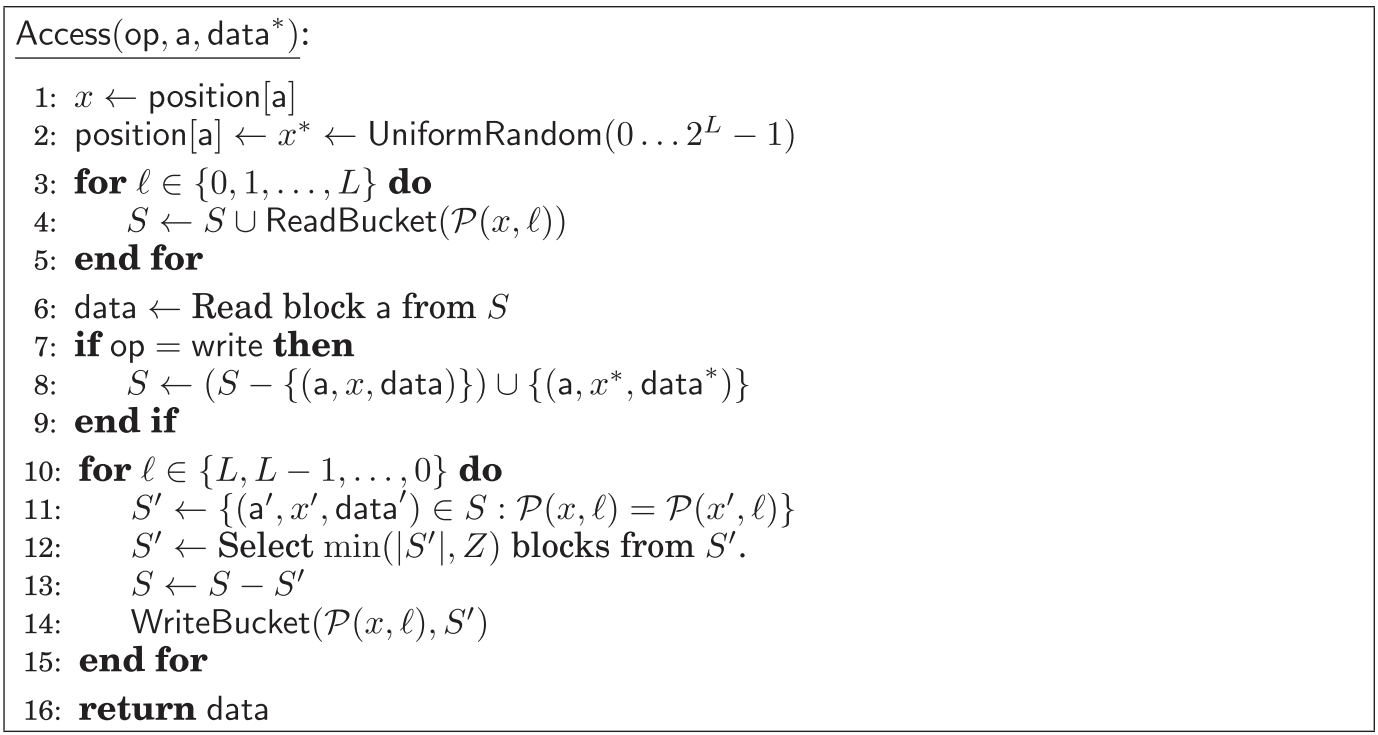
\includegraphics[scale=0.5]{path_oram_pseudocode.png}
    \caption{Pseudocode taken from \cite{stefanov2018path} showing the logic necessary to make an oblivious access in the Path ORAM model}
    \label{fig:pathORAMpseudo}
\end{figure}


\section{Oblivious Dictionary}
\subsection{Operations}
For an oblivious dictionary, we want to support the following operations \cite{wang2014oblivious}:
\begin{itemize}
    \item \textbf{Lookup($k$):} Return the value with key $k$
    \item \textbf{Insert($k, v$):} Insert the value $v$ with key $k$ into the dictionary
    \item \textbf{Delete($k$):} Delete the value with key $k$ from the dictionary
\end{itemize}
Though this oblivious dictionary method can be generalized to include duplicate keys, we will only focus on the case where all keys are unique for the sake of simplicity. Note that ORAM can be viewed as a special case of the dictionary (lookup is a ``read" and insert is a ``write") where the key space is contiguous.

\subsection{Construction}
A naive way to implement dictionaries would be to compile a classic logical tree with ORAM. This would involve giving each element a key alongside its value to generate a logical tree as depicted in Figure \ref{fig:bin_tree}. Even if we assume, for simplicity, that the tree is balanced and static, it's still an inefficient way to make an oblivious dictionary. Instead, we can encode a logical tree \textit{within} the recursion used by Path ORAM itself.

\begin{figure}
\centering
\begin{minipage}{.45\textwidth}
  \centering
  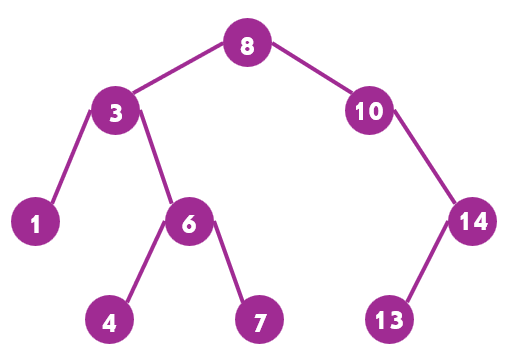
\includegraphics[scale=0.6]{bin_tree.png}
  \captionof{figure}{Naive logical tree compiled with ORAM}
  \label{fig:bin_tree}
\end{minipage}\hfill %
\begin{minipage}{0.45\textwidth}
  \centering
  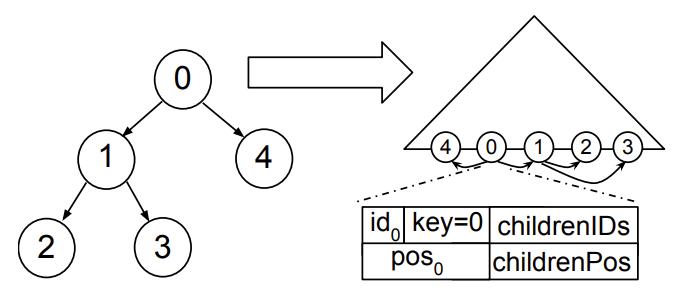
\includegraphics[scale=0.5]{oram_bin_tree.png}
  \captionof{figure}{A diagram representation of a block within the oblivious binary tree \cite{stefanov2018path}}
  \label{fig:oram_bin_tree}
\end{minipage}
\end{figure}

The implementation of a dictionary with binary search trees is simple and intuitive. Each block can be described as containing the following: a key, a value, a pointer to the current block's path, the left key, a pointer to the left child's path, the right key, and a pointer to the right child's path as can be seen in Figure \ref{fig:oram_bin_tree}.


\subsection{Access Protocol}
The only part of the access protocol that differs significantly from the regular setup of Path ORAM is the existence of parents and children. Thus, we must simply maintain the invariant that the parent's child pointers get updated whenever the child's own path is changed on access. This idea can be extended for insertion and deletion in dynamic trees but it remains within the same complexity class for overhead. Beyond that, the access protocol is very similar to the pseudocode shown in Figure \ref{fig:pathORAMpseudo}.

\subsection{Overhead}
The improved oblivious data structure has an overhead of $O(\log^2 n)$ with $O(\log n)$ from the recursion level and $O(\log n)$ from the size of the tree. This is an improvement in contrast to the naive approach that compiles binary searching--which automatically incurs a $O(\log n)$ search cost \cite{gentry2013optimizing}-- with Path ORAM--that already has a $O(\log^2 n)$ lookup cost-- giving an overall $O(\log^3 n)$ overhead.

It is possible to achieve $O(\log n)$ overhead as shown by Asharov et. al. \cite{asharov2023futorama}. With this low overhead, this implementation of an oblivious dictionary finally becomes practical and a viable choice for real-world security. However, there are many restrictions and assumptions that must be met before FuturORAMa can be used and thus some people still prefer to use Path ORAM or Circuit ORAM despite the larger overhead.

\section{Oblivious Stacks / Queues}
\subsection{Operations}
Zahur et. al. also proposes a circuit-based construction of a stack/queue but, for the proof of concept, we will only describe the Path ORAM implementation for stacks \cite{zahur2016revisiting}. Note that oblivious queues can be made in a very similar way. The oblivious stack supports the following operations \cite{toft2011secure}:
\begin{itemize}
    \item \textbf{Push($v$):} Push the value $v$ on the stack
    \item \textbf{Pop():} Pop the top element off the stack and return it
\end{itemize}

\subsection{Construction}
You only need one tree to store a stack. Then, the head pointer holds the path on which the head of the stack resides. Each item holds a value, $v$, a pointer to itself, and a pointer to the next block's path.

\subsection{Access Protocol}
Push simply requires us to choose a path for the new element and then put it onto the stack by setting it to the new head. Pop is very similar and just pops off and removes the current head of the stack.

\subsection{Overhead}
Because there is only one tree and we only need to worry about modifying one element in the tree at a time, each operation takes $O(\log n)$ time. Note that this is a randomized algorithm because there is only one tree and thus this scheme uses non-recursive Path ORAM. We'll learn about a deterministic oblivious algorithm in a later section on oblivious Turing machines.


\section{Oblivious Heaps / Priority Queues}
This oblivious data structure constructed using non-recursive Path ORAM is somewhat similar to that of oblivious stacks and queues but has a few notable differences. For simplicity, we are again assuming that all keys are distinct.

\subsection{Operations}
\begin{itemize}
    \item \textbf{$Extract\_min()$:} Returns the item with the minimum priority
    \item \textbf{$Insert(k, v)$:} Inserts the value $v$ with priority $k$
\end{itemize}

\subsection{Construction}
Using the hierarchical ORAM proposed by Kasper and Larsen, we can store the elements in order with a block containing the the value, a self-referential pointer, a pointer to this subtree minimum's path, and the subtree's minimum itself \cite{larsen2018yes} \cite{asharov2023futorama}. \cite{wang2014oblivious}.

\subsection{Access Protocol}

\subsubsection{Extract-min()}
In extract-min(), we first get the minimum value of this tree, aka the subtree minimum at the root. Let $ptr^*$ denote the path the subtree minimum value resides on. We want to remove the subtree minimum value's record from the path stored in $ptr^*$. To do this, we evict on the path $ptr^*$ and, to maintain correctness, we recalculate the subtree minimum values stored in each node along $ptr^*$'s path. Intuitively, since we're removing the subtree minimum from the path, the subtree minimum of all blocks along that path can change. Note that the subtree minimum of a parent is equal to the minimum between the subtree minimums of its two children, so as long as we update from the leaf node upwards, it only requires $O(\log n)$ overhead.


\subsubsection{Insert(k, v)}
First, we choose a path at random and assign that to the block we want to insert. Then, we add our new block to the root of the tree. Lastly, we perform an eviction on two random paths and recalculate the subtree minimum for each node on the two evicted paths to maintain the correctness property. To maintain the oblivious property, we simply pad either operation such that both operations read the same number of paths. This makes the operations indistinguishable from each other to an outside perspective.

\subsubsection{Other operations}
We can also implement ``$delete(ref)$" where $ref$ is a reference to the pointer we want to delete, and ``$decrease\_key(ref, k')$" where we decrease the key of the value ref is referencing to $k'$. In both these cases, we use references to access the path and ensure that correctness is maintained over the tree.
\begin{itemize}
    \item \textbf{Delete(ref):} Access the path pointer denoted by $ref$, removes the item with key $k$, evicts along the path pointed to by $ref$, and recalculates the subtree minimum for each node along the path
    \item \textbf{Decrease-key(ref, k):} Delete(ref), insert($k', v$)
\end{itemize}

\subsection{Overhead}
As expected, since insertion and extract-min() only require us to update the path the element resides on in linear time, they only incur a $O(\log n)$ overhead.

\section{Oblivious Turing Machines}
\subsection{Operations}
As a reminder, in the oblivious Turing machine model we want to hide whether the Turning machine is going left, right, or staying still on the tape.

\subsection{Construction}
Each level of the structure consists of three ``superblocks" increasing exponentially in size by a power of two (ex: the first level has three superblocks of size 1, the second has three superblocks of size 2, the $i$th level has three superblocks of size $2^i$, and so on) as seen in Figure \ref{fig:turing_blocks}. We denote $HEAD$ to be the head pointer of the Turing machine. We then maintain the following invariant throughout the protocol: When a level is rebuilt--for all except the last $n$th level--HEAD lies in the middle superblock.

\begin{figure}
    \centering
    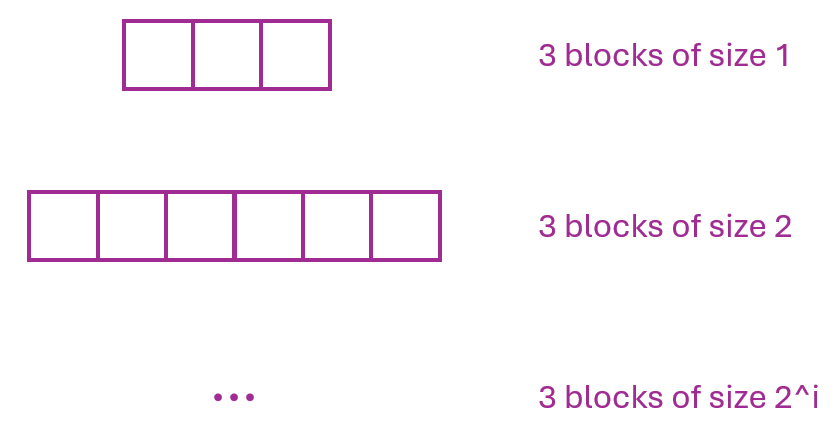
\includegraphics[scale=0.8]{blocks.png}
    \caption{A diagram representation of the levels within an oblivious Turing machine}
    \label{fig:turing_blocks}
\end{figure}

We also want an invariant that indicates how, if level $i$ is updated, all levels $1$ to $(i-1)$ should be notified that $i$ has been updated. The reason for that is each element has multiple copies across levels, thus we must ensure that each copy is updated when the element is updated. This propagation can be done in linear time with respect to the level size.

\subsection{Access Protocol}
The access protocols are easy to implement because a Turing machine can only ``read" or ``write" which can be done with the same access protocol as ORAM as shown in Figure \ref{fig:pathORAMpseudo}.

\subsection{Overhead}
The $i$th level is rebuilt every $2^i$ steps with a rebuilding cost in $O(2^i)$. Thus, over the protocol the costs to rebuild are:
\begin{align*}
    &\textbf{Level 0: } c \cdot 2^0 = c \\
    &\textbf{Level 1: } c \cdot 2^1\cdot \text{ rebuild every 2 steps} \Rightarrow c \cdot 2^0 \text{(amortized)} \tag{Rebuild cost is linear}\\
    &\text{etc } \dots
\end{align*}
At each level we get $c$ work and thus we incur $O(\log n)$ cost per operation. This result is actually quite old and has been proven since Fischer and Pippenger in 1979 \cite{pippenger1979relations}.

\newpage
\bibliographystyle{alpha}
\bibliography{refs.bib}
\end{document}